\subsection{Open-set behaviour: high closed-set accuracy, poor rejection}
\label{sec:openset}

We withhold three classes from training and evaluate on a test set containing all ten, using two holdout configurations: the three 0.021-in faults (classes 3, 6, 9) and the three 0.007-in faults (classes 1, 4, 7). Closed-set accuracy on the known classes stays at 0.97--1.00, i.e.\ the model is as confident as ever; the only way to see the problem is to look at what it does with the three classes it has never seen.

Table~\ref{tab:openset} reports rejection quality. Averaged over the 48 runs, AUROC is 0.90 (range 0.70--1.00) and TPR at 5\% false-acceptance rate is 0.58 (range 0.01--1.00): a quarter of the runs would accept more than half of the unknown faults, and one would accept almost all of them.

\textbf{Finding 7.} Rejection quality is architecture-dependent, unstable across holdout sets, and \emph{anti}-correlated with noise robustness. WDCNN, the most noise-robust model of the eight (0.98 at 10\,dB), has the worst rejection (AUROC 0.84, TPR at 5\% FPR 0.12); ResNet1D and DS-CNN, the two most brittle models in noise, reject best (AUROC 0.97). Across the eight models, Spearman $\rho=-0.64$ ($p=0.09$) links 10\,dB accuracy and mean AUROC---weak, but the opposite of what a deployment-minded reader would expect. The mechanism is visible in the scores: a model that has learned a wide, noise-tolerant decision function maps unknown faults into the interior of a known class, while a brittle model responds with a confidently wrong but \emph{outlying} prediction. A claim that a model is robust in the noise sense should therefore be accompanied by an open-set number, because the two properties are not aligned. Nor can the recommendation of Section~4.3 repair the other axis: the same per-batch augmentation that adds 27 points at 10\,dB lowers mean AUROC from 0.899 to 0.797 (Section~4.7).

\begin{table}[t]
\centering
\caption{Open-set rejection: three of ten classes withheld, two holdout configurations $\times$ three seeds. The best mean AUROC, and the best and the worst mean TPR, are bold.}
\label{tab:openset}
\begin{tabular}{lrrrrrr}
\toprule
& \multicolumn{2}{c}{AUROC} & \multicolumn{2}{c}{TPR at 5\% FPR} & \multicolumn{2}{c}{mean} \\
\cmidrule(lr){2-3}\cmidrule(lr){4-5}\cmidrule(lr){6-7}
model & 3,6,9 & 1,4,7 & 3,6,9 & 1,4,7 & AUROC & TPR \\
\midrule
DS-CNN      & .979 & .965 & .888 & .860 & \best{.972} & .874 \\
ResNet1D    & .967 & .971 & .788 & .871 & .969 & .829 \\
MCNN        & 1.000& .922 & .998 & .617 & .961 & \best{.807} \\
TICNN       & .993 & .822 & .975 & .047 & .908 & .511 \\
ViT1D       & .958 & .841 & .776 & .352 & .900 & .564 \\
MLP-Mixer1D & .988 & .762 & .951 & .068 & .875 & .509 \\
WDCNN       & .829 & .845 & .096 & .145 & .837 & \best{.121} \\
LeNet1D     & .818 & .751 & .544 & .332 & .785 & .438 \\
\bottomrule
\end{tabular}
\end{table}

\begin{figure}[t]
\centering
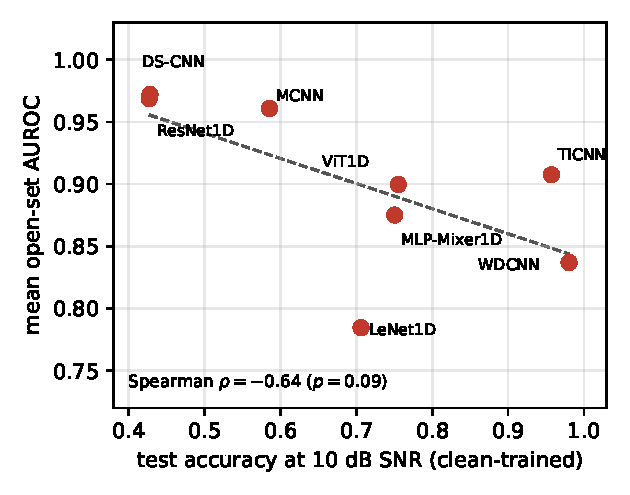
\includegraphics[width=0.62\textwidth]{../figures/fig6_openset.pdf}
\caption{Noise robustness and open-set rejection are not the same property. Each point is one architecture: test accuracy at 10\,dB SNR under clean training (horizontal) against mean open-set AUROC over both holdout configurations (vertical). The two are anti-correlated (Spearman $\rho=-0.64$, $p=0.09$): the model that degrades least under noise rejects unknown faults worst.}
\label{fig:openset}
\end{figure}

\subsection{Can the robustness recipe also buy rejection?}
\label{sec:aug-openset}

Section~4.3 recommends per-batch noise augmentation, and it is the cheapest
intervention in the paper: free in parameters, worth 27 points at 10\,dB. If robustness and
rejectability were two faces of the same smoothing effect, the same one-line change should
also improve rejection. We repeated both holdout configurations with augmented training
(32 runs, two seeds, everything else as in Section~4.6).

Table~\ref{tab:opensetaug} reports the result: it does not. Mean AUROC falls from 0.899 to
0.797 and mean TPR at 5\% FPR from 0.570 to 0.388, and only 4 of the 32 paired
(model, holdout, seed) configurations improve in AUROC; a paired Wilcoxon signed-rank test
gives $p=5\times10^{-7}$ for AUROC and $p=6\times10^{-3}$ for TPR (Holm-corrected over the two
metrics). The two models that do improve slightly are WDCNN and LeNet1D, the two whose
clean-trained rejection was already the worst. The model that loses most is DS-CNN, the best
rejector of the clean-trained set (AUROC 0.972): it drops to 0.644 while its 0\,dB accuracy
climbs from 0.228 to 0.620. The two axes are not merely uncorrelated; on this evidence they
trade off.

\begin{table}[t]
\centering
\caption{Open-set rejection under noise-augmented training (32 runs, two
seeds). $\Delta$ is relative to the clean-trained model on the same holdout configurations
(Table~\ref{tab:openset}); means are over the eight models. In each of the four metric columns the best value is bold.}
\label{tab:opensetaug}
\begin{tabular}{lrrrrrr}
\toprule
& \multicolumn{3}{c}{mean AUROC} & \multicolumn{3}{c}{mean TPR at 5\% FPR} \\
\cmidrule(lr){2-4}\cmidrule(lr){5-7}
model & clean & +aug & $\Delta$ & clean & +aug & $\Delta$ \\
\midrule
WDCNN       & .837 & .822 & $-0.015$ & .121 & .173 & $+0.052$ \\
TICNN       & .908 & .833 & $-0.075$ & .511 & .338 & $-0.173$ \\
MCNN        & .961 & .846 & $-0.115$ & .807 & .541 & $-0.267$ \\
ResNet1D    & .969 & \best{.857} & $-0.112$ & .829 & \best{.548} & $-0.281$ \\
DS-CNN      & \best{.972} & .644 & $-0.328$ & \best{.874} & .173 & $-0.702$ \\
LeNet1D     & .785 & .743 & $-0.041$ & .438 & .463 & $+0.025$ \\
ViT1D       & .900 & .829 & $-0.070$ & .564 & .393 & $-0.171$ \\
MLP-Mixer1D & .875 & .798 & $-0.077$ & .509 & .473 & $-0.036$ \\
\midrule
mean        & .899 & .797 & $-0.103$ & .570 & .388 & $-0.182$ \\
\bottomrule
\end{tabular}
\end{table}

The mechanism is the one described in Section~5.3: augmentation
widens the region a class occupies in score space, which is exactly what makes the model
tolerant to perturbation and exactly what makes an unseen fault land inside a known class.
Training and evaluation therefore pull the two objectives in opposite directions, and a
practitioner who needs both must decide it at the decision layer rather than in the recipe.
Section~4.8 tests whether the decision layer can supply what the recipe removes.
\subsection{Score choice, not the training recipe, explains the rejection gap}
\label{sec:scores}

Section~4.7 measured rejection with the softmax maximum. That is a read-out of a trained network
rather than part of it: two networks with the same class geometry can rank unknown faults
differently depending on how their confidence is summarised, and a smoothing operator such as
noise augmentation flattens the softmax distribution in particular. We therefore repeated the
whole open-set grid---eight models, two holdout sets, two seeds, clean and augmented, 64
runs---and scored every trained network three ways after training: the softmax maximum (the
baseline of Sections~4.6--4.7), the negative free energy $T\log\sum_j e^{z_j/T}$, and the
negative minimum Mahalanobis distance to class-conditional Gaussians fitted on the training
logits with a shared covariance. None of the three adds a parameter or a training step; they
differ only in how the logit vector is summarised.

Table~\ref{tab:scores} reports the outcome. Energy is not the answer: it matches or slightly
trails the softmax maximum (mean AUROC 0.889 against 0.899 clean-trained,
$p_{\mathrm{Holm}} = 0.06$; 0.785 against 0.796 augmented). The distance-based score is: mean
AUROC rises from 0.899 to 0.953 on clean-trained models (26 of the 32 paired configurations
improve, $p_{\mathrm{Holm}} = 1.3\times10^{-4}$) and from 0.796 to 0.940 on augmented ones (31
of 32, $p_{\mathrm{Holm}} = 2\times10^{-9}$); mean TPR at 5\% FPR rises from 0.570 to 0.785 and
from 0.387 to 0.746. The augmentation penalty measured in Section~4.7 therefore shrinks by
almost an order of magnitude: 0.103 AUROC and 0.182 TPR with the softmax maximum, 0.013 and
0.039 with the Mahalanobis score.

The reading is consistent with Section~5.3. A softmax maximum measures where a point sits
relative to the decision boundary, so any smoothing of the decision surface---exactly what
augmentation trains---lowers it; the class-conditional structure in logit space survives the
smoothing, and normalising the distance by the spread each class acquires during training keeps
unknown faults far from all class centres. Despite its lower average AUROC, the augmented model
scored with Mahalanobis (0.940) still beats the clean-trained model scored with the softmax
maximum (0.899) on the same runs. The trade-off of Section~4.7 is thus partly a property of the
read-out rather than of the features: the information that separates unseen faults is still
there after augmentation, and the maximum-probability summary loses it.

Two cautions. First, the gain could belong to the coordinate system rather than to the
read-out: logits are a contraction of the features, and a distance in a contracted space need
not behave like a distance in the space it contracts. We therefore repeated the grid with the
same estimator fitted to the input of the last linear layer (penultimate features, 32--256
dimensions across the eight models, obtained by one uniform rule with no architecture-specific
hook). Mean AUROC is 0.952 clean-trained and 0.938 augmented---indistinguishable from the
logit-space values (paired over 32 configurations: $-0.001$ and $-0.002$ AUROC, $p = 0.95$ and $p = 0.64$)
and still far above the softmax maximum (0.899 and 0.796)---and the augmentation penalty is
again 0.014 AUROC instead of 0.103. What matters is that the score measures distance rather
than probability mass, not the coordinates in which it is measured. Second, the score is a free
parameter of the evaluation, so an open-set number means little without it: the same networks
that look damaged by augmentation under one score look almost unaffected under another, just as
a robustness claim means little without naming the noise family. A reconstruction-based score
remains untested.

\begin{table}[t]
\centering
\caption{Decision-layer scores on the same trained networks (eight models, two holdout sets, two seeds; each cell averages four runs). softmax is the maximum softmax probability used in Sections~4.6--4.7, energy is the negative free energy $T\log\sum_j e^{z_j/T}$, and Mahalanobis is the negative minimum distance to class-conditional Gaussians fitted on the training logits with a shared covariance. All three are computed after training and add no parameters; a fourth read-out, the same distance in penultimate-feature space, is reported in the text. The best score in each row is bold for AUROC and for TPR separately.}
\label{tab:scores}
\begin{tabular}{llrrrrrr}
\toprule
& & \multicolumn{3}{c}{AUROC} & \multicolumn{3}{c}{TPR at 5\% FPR} \\
\cmidrule(lr){3-5}\cmidrule(lr){6-8}
model & training & softmax & energy & Mahalanobis & softmax & energy & Mahalanobis \\
\midrule
WDCNN & clean & .858 & .858 & \best{.938} & .158 & .210 & \best{.670} \\
 & aug & .822 & .819 & \best{.933} & .173 & .224 & \best{.604} \\
TICNN & clean & .904 & .898 & \best{.969} & .508 & .503 & \best{.827} \\
 & aug & .833 & .808 & \best{.962} & .337 & .296 & \best{.774} \\
MCNN & clean & .974 & .961 & \best{.982} & .878 & .794 & \best{.928} \\
 & aug & .846 & .855 & \best{.972} & .540 & .604 & \best{.887} \\
ResNet1D & clean & .965 & .941 & \best{.979} & .793 & .650 & \best{.905} \\
 & aug & .857 & .831 & \best{.970} & .548 & .490 & \best{.839} \\
DS-CNN & clean & .968 & .937 & .968 & \best{.863} & .694 & .858 \\
 & aug & .644 & .628 & \best{.932} & .172 & .154 & \best{.775} \\
LeNet1D & clean & .763 & .794 & \best{.946} & .385 & .523 & \best{.746} \\
 & aug & .743 & .713 & \best{.952} & .463 & .390 & \best{.779} \\
ViT1D & clean & .887 & .882 & \best{.907} & .484 & .455 & \best{.641} \\
 & aug & .829 & .834 & \best{.882} & .393 & .451 & \best{.576} \\
MLP-Mixer1D & clean & .873 & .841 & \best{.932} & .490 & .428 & \best{.705} \\
 & aug & .798 & .792 & \best{.917} & .473 & .353 & \best{.734} \\
\midrule
\textit{mean} & clean & .899 & .889 & \best{.953} & .570 & .532 & \best{.785} \\
 & aug & .796 & .785 & \best{.940} & .387 & .370 & \best{.746} \\
\bottomrule
\end{tabular}
\end{table}

\textbf{Finding 8.} Rejection quality depends on the score as much as on the architecture. The
same trained networks move from 0.899 (softmax, clean) and 0.796 (softmax, augmented) to 0.953
and 0.940 mean AUROC when the rejection score is a logit-space Mahalanobis distance, with no
retraining and no parameters, and the cost of noise augmentation on rejection falls from 0.103
to 0.013 AUROC. A fourth read-out, the same distance in penultimate-feature space, reproduces
both numbers (0.952 and 0.938), so the gain comes from measuring distance rather than from
logit coordinates. A claim that an intervention breaks or preserves rejectability must name the
score it was measured with, exactly as a robustness claim must name the noise family (Finding~9).

\subsection{Other noise families}
\label{sec:noisetypes}

White Gaussian noise is the field's default probe, but real bearing signals also carry impulsive (tonal), harmonic (electrical interference) and drift (sensor or thermal) disturbances. Table~\ref{tab:noisefam} repeats the 10\,dB and 0\,dB evaluation with three such families, using the four models that span the range of our results; the families are defined in Section~3.4 and the clean-trained Gaussian column is repeated for reference.

Three things change. First, broadband Gaussian noise turns out to be the \emph{hardest} of the four families for the two narrow-kernel CNNs, but not for the other two: under impulsive noise ResNet1D and DS-CNN reach 0.970 and 0.995 at 10\,dB, i.e.\ 54 and 57 points above their own Gaussian accuracy, and at 0\,dB DS-CNN keeps 0.929 against 0.228. Sparse transients are statistically closer to the impulsive excitation of a bearing fault than broadband noise is, so there is nothing to suppress. Second, \emph{low-frequency drift} is the one family that separates the models sharply: ViT1D falls 28 points below its Gaussian level (0.474) and DS-CNN reaches only 0.545, while WDCNN loses nothing under drift (0.993 at 10\,dB, 20 points above its Gaussian level) and ResNet1D gains 33 points. This is the band-pass reading of Section~4.4 again: a wide first kernel removes slow wander, a narrow one maps it onto the fault bands. Third, the ordering induced by the four families is different in every case: DS-CNN is the best model under impulsive noise and among the worst under drift, WDCNN is first under harmonic and drift interference but is beaten under impulsive noise (second at 10\,dB, third at 0\,dB), and the Gaussian order (WDCNN $>$ ViT1D $>$ DS-CNN $>$ ResNet1D) survives in none of them.

\textbf{Finding 9.} A single Gaussian probe does not identify a robust model. Which noise family hurts most is architecture-dependent---drift for ViT1D, broadband Gaussian for the two narrow-kernel CNNs, and for WDCNN no single family is decisive (0.952--0.993 across the four)---the ranking it induces changes with the family, and a robustness claim that does not name the family is unfalsifiable. We also note one instability that a single seed would hide: WDCNN under drift at 0\,dB averages 0.60 with a standard deviation of 0.33 across two seeds, so its apparent robustness there is not reliable.

\begin{table}[t]
\centering
\caption{Architectures under four noise families (clean training, noise at test time only, mean over 2 seeds for the non-Gaussian families and 3 seeds for Gaussian). Accuracy at 10\,dB and 0\,dB SNR.}
\label{tab:noisefam}
\begin{tabular}{lrrrr|rrrr}
\toprule
& \multicolumn{4}{c@{}}{10\,dB SNR} & \multicolumn{4}{c}{0\,dB SNR}\\
model & Gaussian & harmonic & impulse & drift & Gaussian & harmonic & impulse & drift\\
\midrule
WDCNN    & \best{.980} & \best{.952} & .980 & \best{.993} & \best{.405} & \best{.412} & .447 & \best{.604}\\
ResNet1D & .427 & .632 & .970 & .758 & .136 & .183 & .444 & .183\\
DS-CNN   & .428 & .611 & \best{.995} & .545 & .228 & .197 & \best{.929} & .188\\
ViT1D    & .755 & .745 & .887 & .474 & .271 & .258 & .754 & .184\\
\bottomrule
\end{tabular}
\end{table}

\subsection{Efficiency}
\label{sec:efficiency}

Table~\ref{tab:eff} reports parameter counts and measured latency on the same accelerator used for training. The parameter range spans 250$\times$ (3{,}018 to 747{,}722), yet at batch size 1 the wall-clock latency spans only 0.5--5.3\,ms, and at batch size 256 the per-sample cost is 0.009--0.27\,ms, i.e.\ 3{,}750--114{,}000 windows per second. For a monitoring application that processes one window per second per machine, every architecture in this study is over three orders of magnitude faster than needed.

\textbf{Finding 10.} Parameter count does not predict latency, and neither predicts robustness. The two most noise-robust models (WDCNN, TICNN) are also the two fastest at large batch (115k and 49k windows/s), while MCNN, which is 5$\times$ larger than WDCNN and 64$\times$ larger than LeNet1D, is the slowest. Accuracy-per-parameter, the objective that most lightweight-architecture papers optimise, is therefore the wrong objective for this task: the compute budget is not binding, so the only thing that matters is behaviour under the conditions that actually occur---noise and unseen faults.

\begin{table}[t]
\centering
\caption{Parameters and inference latency on the training accelerator (Apple M5, MPS, 1{,}024-sample windows; mean of 30 (batch 1) / 10 (batch 256) forward passes after warm-up). Latencies were measured while other training jobs shared the device, so absolute numbers are 2--3$\times$ pessimistic; relative comparisons are unaffected.}
\label{tab:eff}
\begin{tabular}{lrrrrr}
\toprule
model & params & 1$\times$1024 (ms) & 256$\times$1024 (ms) & ms/window & windows/s \\
\midrule
LeNet1D     & 3{,}018   & 0.50  & 6.65  & 0.026 & 38{,}472 \\
WDCNN       & 34{,}410  & 1.99  & 2.23  & 0.009 & \best{114{,}605} \\
DS-CNN      & 69{,}642  & 4.21  & 17.94 & 0.070 & 14{,}271 \\
TICNN       & 83{,}914  & 1.81  & 5.25  & 0.021 & 48{,}799 \\
ViT1D       & 139{,}850 & 4.59  & 42.90 & 0.168 & 5{,}968 \\
MCNN        & 184{,}554 & 4.23  & 51.42 & 0.201 & 4{,}979 \\
ResNet1D    & 241{,}322 & 5.27  & 31.03 & 0.121 & 8{,}249 \\
MLP-Mixer1D & 747{,}722 & 3.52  & 68.21 & 0.266 & 3{,}753 \\
\bottomrule
\end{tabular}
\end{table}

Table~\ref{tab:cost} summarises the cost of the interventions instead. Noise augmentation is free in parameters and buys 49 points at 10\,dB; the wide stem costs 2{,}608 parameters (1.1\% for ResNet1D) and buys 55; together they buy 56 points at 10\,dB and 73 at 0\,dB for 1.4 points of clean accuracy. No architecture in our set buys anything comparable for a similar price.

\begin{table}[t]
\centering
\caption{Cost of the interventions studied in this paper, measured on one fixed architecture (ResNet1D, 241{,}322 parameters, three seeds). $\Delta$columns are percentage points with respect to the plain model.}
\label{tab:cost}
\begin{tabular}{lrrrr}
\toprule
intervention & $\Delta$params & $\Delta$clean & $\Delta$10\,dB & $\Delta$0\,dB\\
\midrule
noise augmentation          & $0$      & $-11.1$ & $+49.0$ & $+29.3$\\
wide stem $k128c8$          & $+1.1\%$ & $-1.1$  & $+54.6$ & $+32.7$\\
stem + augmentation         & $+1.1\%$ & $-1.4$  & $\best{+56.2}$ & $\best{+72.9}$\\
re-architecture (six variants) & $\pm$ & $-0.1$ to $-4.3$ & $0$ to $+13$ & --\\
\bottomrule
\end{tabular}
\end{table}

\subsection{Second dataset: Paderborn}
\label{sec:paderborn}

To check that the conclusions are properties of the evaluation rather than of CWRU, we repeat the noise stress on Paderborn bearing data \citep{lessmeier2016paderborn}, using the two classes available in the subset we downloaded (healthy, outer race) and the same windowing, split, training and noise pipeline.

We use the 18-bearing KAt subset (six healthy bearings K001--K006 and twelve with artificial outer-race damage), 60,000 training and 20,000 test windows, and the same four models and noise pipeline, with and without SNR~$\mathcal{U}[0,15]$ augmentation (Table~\ref{tab:paderborn}).

Clean accuracy is again compressed, though at a different level: the four plain models span 0.962 to 0.990, i.e.\ 3 points. Under noise they separate: at 10\,dB the plain models fall to 0.838--0.908 (7 points), at 5\,dB to 0.675--0.851 (18 points) and at 0\,dB to 0.517--0.807 (29 points). The absolute loss is smaller than on CWRU---Paderborn is a harder two-class problem that is not saturated to 99\% even clean---but the mechanism is the same, and on the harder condition the models that look equally good clean differ by 29 points.

The rank inversion reappears in a weaker form (plain rows). ResNet1D is the best model clean (0.990) and drops to third at 10\,dB (0.885) and to second-worst at 0\,dB (0.558, 23 points below WDCNN); DS-CNN is third clean (0.974) and last at both 10\,dB (0.838) and 0\,dB (0.517). The clean and noisy orderings of the four plain models share no pair (Spearman $\rho=0$). The inversion is thus directional rather than complete: WDCNN, the worst model clean, is second at 10\,dB, but TICNN is first in both conditions, so we cannot claim a full reversal on this dataset.

Augmentation behaves as it does on CWRU, and it is not free: it costs 6.6 points of clean accuracy for WDCNN and 13--15 points for the other three, and buys 1.6--5.1 points at 10\,dB, 9.3--24.7 at 5\,dB and 25.2 at 0\,dB for ResNet1D and DS-CNN. Most informative, the eight augmented rows have the \emph{same} clean and noisy ordering (WDCNN $>$ ResNet1D $>$ TICNN $>$ DS-CNN at both 10\,dB and clean), i.e.\ the inversion disappears once the perturbation is part of the training distribution. We note that TICNN with augmentation has a large seed spread (clean $0.826\pm0.083$) and loses 0.8 points at 0\,dB, so the three-model picture is more stable than the four-model one.

\textbf{Finding 11.} The collapse under noise and the failure of clean accuracy to predict it reproduce on a second rig (two datasets, two label spaces, two window lengths): the clean-best model falls to third at 10\,dB and to second-worst at 0\,dB, and the clean-worst model is not the noisy-worst. The inversion is weaker than on CWRU---TICNN leads in both conditions---but it disappears under augmentation in the same way, so the phenomenon is a property of clean training rather than of one dataset.

\begin{table}[t]
\centering
\caption{Paderborn (two classes, 60k/20k windows), mean$\pm$std over two seeds. \emph{plain}: trained clean; \emph{aug}: trained with SNR~$\mathcal{U}[0,15]$ per batch. Noise is added at test time only. Best value of each column within each training mode in bold.}
\label{tab:paderborn}
\begin{tabular}{llcccc}
\toprule
model & training & clean & 10\,dB & 5\,dB & 0\,dB\\
\midrule
WDCNN    & plain & .962$\pm$.002 & .899$\pm$.000 & .843$\pm$.002 & .789$\pm$.007\\
         & aug   & \best{.896}$\pm$.005 & \best{.941}$\pm$.005 & .937$\pm$.002 & .814$\pm$.017\\
TICNN    & plain & .976$\pm$.000 & \best{.908}$\pm$.003 & \best{.851}$\pm$.012 & \best{.807}$\pm$.019\\
         & aug   & .826$\pm$.083 & .924$\pm$.049 & .944$\pm$.018 & .800$\pm$.040\\
ResNet1D & plain & \best{.990}$\pm$.000 & .885$\pm$.024 & .769$\pm$.005 & .558$\pm$.013\\
         & aug   & .856$\pm$.019 & .936$\pm$.007 & \best{.951}$\pm$.008 & \best{.811}$\pm$.001\\
DS-CNN   & plain & .974$\pm$.001 & .838$\pm$.010 & .675$\pm$.032 & .517$\pm$.006\\
         & aug   & .822$\pm$.026 & .884$\pm$.030 & .922$\pm$.012 & .769$\pm$.017\\
\bottomrule
\end{tabular}
\end{table}

\section{Discussion}

\subsection{Why the benchmark cannot see the difference}
CWRU clean test accuracy has been at the ceiling for years, and every model in our set sits within 3 points of it. A metric that is bounded above by 100\% and is already at 97--100\% has almost no dynamic range left: the differences that remain are within three seeds of the same model, and within the variance of optimiser luck. The natural conclusion is not that the models are equally good but that \emph{clean CWRU accuracy has stopped carrying information}. Any paper that reports it as evidence of progress is reporting noise.

\subsection{Two different robustness mechanisms}
Our ablation separates two mechanisms that the literature usually conflates. The first is a training-distribution effect: exposing the model to noisy inputs makes it invariant to them, and this alone is worth $+26.8$ points at 10\,dB averaged over eight architectures. The second is an architectural effect: a wide multi-channel front-end maps the raw window through a bank of learnable band-pass filters before the backbone sees it, which is worth up to $+52$ points for a narrow-kernel backbone and essentially nothing for a backbone that already mixes the whole window. The two are complementary but not equivalent: on the same backbone the stem costs 1.1 points of clean accuracy where augmentation costs 11.1, the stem adds 1.1\% of the parameters, and augmentation is free in parameters but still helps the models the stem cannot fix.

That a wide first kernel helps under noise is not new—WDCNN made it standard in 2017—but our results show that the effective part of the design is the \emph{number of parallel channels}, not the kernel width. A single 64-sample kernel adds only 66 parameters and buys $+34$ points at 10\,dB but destroys clean accuracy, because one filter has to serve every fault frequency. Eight parallel filters at the same width cover several resonance bands at once, which is what the clean-accuracy recovery in Table~\ref{tab:stem} measures. Widening the kernel further adds little: $k=128$ buys another 2.7 points for 24\% more parameters.

There is a physical reading of this. At 12\,kHz, 64 samples span 5.3\,ms; the ball-pass frequencies of a 6205-2RS bearing at the CWRU speeds are roughly 107\,Hz (BPFO, 9.3\,ms) and 162\,Hz (BPFI, 6.2\,ms) \citep{randall2011tutorial}. A single wide kernel is comparable to one period of the fault signature, so it can act as a matched filter for one resonance band only; a bank of them covers several. Noise, which is broadband, is suppressed by the band-pass character while the periodic fault signature passes.

\subsection{Robustness and rejectability are different axes}
Our open-set audit adds a third inversion to the one described in Section~4.2. A model can be robust to additive noise---because its front end averages over many samples, or because it was trained to ignore perturbation---and yet be unable to tell a fault it has never seen from one it has. The two properties are weakly anti-correlated in our data ($\rho=-0.64$): the models with the widest effective receptive field and the most noise-tolerant decision functions (WDCNN, TICNN) are the ones that map unknown faults into the interior of a known class.

This is not a paradox. A noise-tolerant classifier is by construction a smoothing operator: it is trained to give the same answer for many perturbations of the input, and an unknown fault class is just one more perturbation that falls inside the smoothed region. Rejection quality instead depends on how \emph{peaked} the score function is around the training classes, which is what narrow, brittle models have. The practical consequence is that the two requirements must be evaluated, and optimised, separately: reporting a noise-robust model as deployment-ready without an open-set number conflates two axes of behaviour.

How much of the second axis is the score is a separate question, and Section~4.8 answers it: with a Mahalanobis distance score the same networks reach 0.953 (clean) and 0.940 (augmented) mean AUROC (0.952 and 0.938 when the distance is measured in penultimate-feature space), and the cost of augmentation falls from 0.103 to 0.014 AUROC. The trade-off of Section~4.7 is therefore mostly a property of the softmax read-out: the smoothing that buys noise tolerance flattens the maximum-probability summary, but the class-conditional geometry that separates unseen faults survives it. The practical rule is the same as for robustness claims---report the open-set number together with the score that produced it.

\subsection{What a practitioner should do}
Given a fixed budget and a narrow-kernel backbone, our results suggest a concrete ordering: (i) add per-batch noise augmentation, which is free in parameters and worth 27 points on average; (ii) add a wide multi-channel stem, which is worth up to 55 points for about 1\% more parameters; (iii) only then consider architectural novelty. Both interventions are implemented in a few lines (Appendix~A). Reporting should follow with the test matrix that produced these numbers: at minimum clean plus two noisy SNRs, with seeds and paired statistics.

\subsection{Implications for evaluation practice}
A reviewer cannot detect a 55-point robustness gap from a table of clean accuracies, and an author has no incentive to report a stress test that might show a smaller number. The fix is structural rather than technical: noise stress and open-set evaluation should be mandatory in the reporting checklist, the way top conferences in vision now require multi-seed results. We give a seven-item list in Appendix~A.

\subsection{Relation to prior critique}
Recent position papers argue that vibration benchmarks are contaminated by overlapping-window leakage and non-comparable splits \citep{phme2026,ssrn2024}. Our audit agrees on the protocol problem but finds the effect small: at most 0.6 points at full data and at most 0.9 in a 20-per-class regime. The more serious contamination is saturation: when every method scores 99\%, the protocol no longer matters because the metric has no resolution. Our contribution is to show what a resolution-restoring test looks like and what it reveals.

\section{Limitations}

Our study has clear limits, and we state them rather than hide them behind a robustness claim.

\paragraph{Datasets.} Both datasets are laboratory test rigs with a handful of bearings, constant speed and controlled loads. The Paderborn subset we use contains artificial damage on the outer race only, so it supports a two-class healthy/outer task rather than a full three-class diagnosis; it tests the evaluation method, not the label space. Real machines have varying speed, time-varying load, multiple sensors and long-term drift. Noise is additive and white in our main matrix; while we check two other families, we do not simulate sensor faults, missing samples or non-stationarity.

\paragraph{Models.} Eight architectures is a sample, not a census. We exclude transformer hybrids, graph networks and domain-adaptation methods, and we deliberately do not tune per-architecture hyperparameters, so we cannot claim that any architecture is at its best. Conversely, the "identical harness" design means differences are lower bounds on what tuning could buy.

\paragraph{Noise protocol.} SNR is defined on the raw window before normalisation, per window, with a fixed noise realisation per evaluation; we do not average over noise realisations, which would narrow the error bars. The augmentation schedule (uniform 0--15\,dB per batch) is one of many; we did not search it.

\paragraph{Open set.} Two held-out-class configurations (three of ten), and the rejection score in the main audit is the softmax maximum. We do compare three alternatives on the same networks (Section~4.8): the negative free energy behaves like the softmax maximum, while a Mahalanobis distance improves mean AUROC from 0.899 to 0.953 clean-trained and 0.796 to 0.940 augmented in logit space and to 0.952 and 0.938 in penultimate-feature space, leaving an augmentation cost of 0.013--0.014 AUROC; a reconstruction-based score remains untested. The large spread across holdout configurations (0.05--0.87 TPR at 5\% FPR for the same model) also means that a single open-set number should be read as a sample, not as a property.

\paragraph{Randomness in augmentation.} The noise schedule draws a fresh SNR per mini-batch. In the code released with this paper the draw is derived from the seed, so a run is exactly reproducible; the augmented results reported here were produced before that fix, so re-running an augmented configuration reproduces it to within 1--8 points at 10 and 5\,dB (the random draws differ). All augmented numbers in this paper are means over three seeds, and the standard deviations in Table~\ref{tab:combo} include this variation. The claims we draw from them are differences of 20--50 points.

\paragraph{Statistical scope.} Three seeds, one data ordering, one hardware platform. Paired tests control for model and seed but not for the choice of split, which we leave to future work as a variance component.

\section{Conclusion}

The field's standard benchmark has saturated, and the standard robustness probe is not comparable across papers. We re-evaluated eight lightweight 1D architectures under one leakage-safe harness and found that clean accuracy is uninformative while noise accuracy separates the same models by 55 points; that the separation is mostly a property of the training recipe, which a one-line per-batch noise augmentation repairs; that a multi-channel wide front-end recovers up to 52 points for about 1\% more parameters, with the number of channels rather than the kernel width as the decisive knob; and that open-set rejection varies from 0.12 to 0.87 TPR at 5\% FPR across architectures even when closed-set accuracy is near 100\%, with the most noise-robust model rejecting worst---an axis that the augmentation repairing noise accuracy pushes the other way (AUROC 0.90 to 0.80) unless the rejection score is chosen with it, in which case almost all of that loss is recovered (0.80 to 0.94 with a Mahalanobis distance score, in logit or penultimate-feature space). The practical message is short: stop reporting clean CWRU accuracy as evidence, report a noise matrix and an open-set number, and prefer a recipe change to an architecture change.

\section*{Funding}
This research received no external funding.

\section*{Conflict of interest}
The author declares no competing interests.

\section*{Data and code availability}
All splits, per-seed result files, figures and the exact commands that regenerate every number in this paper are released with the manuscript. CWRU and Paderborn data are public and are not redistributed.

\appendix
\section{Reproduction commands and reporting checklist}

\paragraph{Reproduction.} From the released repository, the following commands regenerate the paper:
\begin{enumerate}
\item \texttt{python -m code.data.cwru} --- build the four split protocols and verify zero sample overlap.
\item \texttt{python -m experiments.grid --grid e2\_noise\_clean --seeds 0,1,2 --epochs 20}
\item \texttt{python -m experiments.grid --grid e4\_aug --seeds 0,1,2 --epochs 20}
\item \texttt{python -m experiments.grid --grid e3\_openset --seeds 0,1,2 --epochs 20}
\item \texttt{python -m experiments.stem\_probe} --- the wide-stem ablation.
\item \texttt{python -m experiments.e6\_noise\_types} --- harmonic, impulsive and drift noise.
\item \texttt{python -m experiments.e7\_efficiency} --- parameters and latency.
\item \texttt{python -m experiments.grid --grid e0\_sat --seeds 0,1 --epochs 20} --- the four split protocols used in Table~\ref{tab:sat}.
\item \texttt{python experiments/e0\_fewshot.py --seeds 0,1} --- the few-shot leakage audit.
\item \texttt{python -m experiments.e8\_paderborn} --- the second dataset (Paderborn).
\item \texttt{python -m experiments.e9\_openset\_aug --seeds 0,1 --epochs 20} --- rejection under augmented training (Section~4.7).
\item \texttt{python -m experiments.e10\_scores --seeds 0,1 --epochs 20} --- the three rejection scores (Section~4.8).
\item \texttt{python -m experiments.e11\_penultimate --seeds 0,1 --epochs 20} --- the same grid scored in penultimate-feature space.
\item \texttt{python -m experiments.stats \&\& python -m experiments.figures} --- tables and figures.
\item \texttt{python experiments/check\_tables.py} --- re-verifies every table in this manuscript cell by cell against \texttt{results/*.json}.
\end{enumerate}
A single training run takes 8--84\,s on a laptop-class accelerator (Apple M5, MPS backend); the full matrix is about 430 runs, i.e.\ a few hours.

\paragraph{Reporting checklist.} We suggest that every vibration-diagnosis paper report:
\begin{enumerate}
\item the split protocol, at recording level, with the number of shared sampling points between train and test (ideally zero, verified);
\item clean accuracy \emph{and} accuracy at at least two SNRs, with the noise model and the SNR definition;
\item at least three seeds, with mean and standard deviation, and paired statistics for any claimed improvement;
\item parameter count and inference latency at the intended batch size;
\item open-set behaviour when the deployment scenario can encounter unseen faults (AUROC and TPR at a fixed FPR);
\item whether the training set was noise-augmented, and the augmentation schedule;
\item code and split files, or an explicit statement that they are unavailable.
\end{enumerate}

\bibliographystyle{unsrt}
\bibliography{refs}

\end{document}
